\section{Solution}\label{chapter:Solution}
This section covers the solution of the exercise. We continued on the work done in the
previous exercise. This included VHDL files for a MIPS multi cycle processor, that 
simulated well in software, but had some trouble with branching when it came to 
running on an FPGA. The work was mainly in implementing and connecting the different 
pipeline registers with control signals, including the \textit{hazard detection unit}
and the \textit{forwarding unit}.

\subsection{Assignment}
The assignment was \textbf{Extend the processor from the previous assignment by changing the 
data path to a pipeline}, the including tasks were to

\begin{itemize}
  \item Add pipeline registers to all the stages described in Figure \ref{pipeline-registers}.
  \item Optimize performance by adding data-forwarding techniques to the pipeline.
  \item Optimize performance by adding hazard-detection techniques
\end{itemize}
The assignment also specified that at least the following instructions from 
the MIPS Architecture should be implemented

\begin{description}
  \item[ALU] \hfill \\
    ADD - Addition \\
    SUB - Subtraction \\
    SLT - Set on Less than \\
    AND - Logical and \\
    OR - Logical or
  \item[Conditional] \hfill \\
    BEQ - Branch when equal
  \item[Immediate] \hfill \\
    LW - Load Word \\
    SW - Store Word \\
    LUI - Load Upper Immediate
\end{description}

\subsection{Architecture}
The architecture for the assignment is shown in Figure \ref{pipeline-registers}.
This is the same architecture that is described in the course 
text book\cite{patterson-hennesay}, throughout chapter 4.
The architecture, extended with hazard detection and forwarding is shown in
Figure \ref{mips-architecture}.

\begin{figure}[!ht]
    \centering
        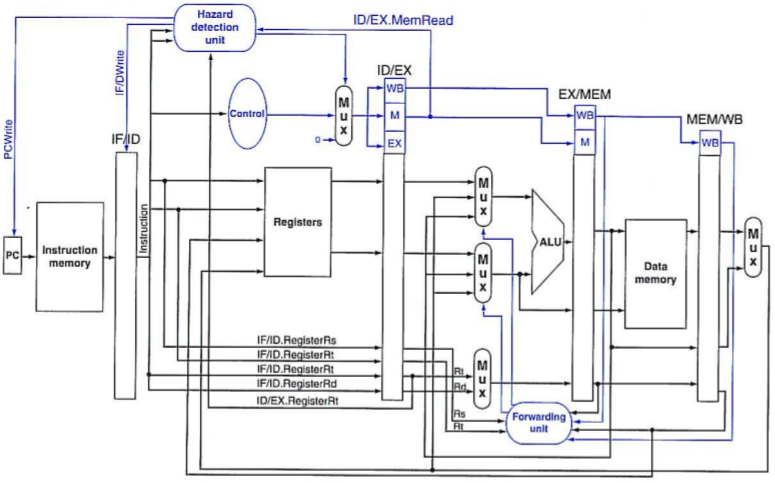
\includegraphics[width=1\textwidth]{figures/mips-pipeline}
        \caption{MIPS pipeline architecture, with hazard detection and data forwarding}
    \label{mips-architecture}
\end{figure}

\subsection{Project files}
The project consisted of the following modules from the last assignment

\begin{itemize}
    \item Com.vhd \hfill \\
        \textit{Communication module, used for programming and controlling the FPGA}
    \item memory.vhd \hfill \\
        \textit{Data memory module}
    \item register\_file.vhd \hfill \\
        \textit{Register module}
    \item alu.vhd \hfill \\
        \textit{Arithmetical Logical Unit}
    \item control\_unit.vhd \hfill \\
        \textit{The main control unit}
    \item alu\_control.vhd \hfill \\
        \textit{ALU control unit}
    \item pc\_register.vhd \hfill \\
        \textit{Program Counter module}
    \item processor.vhd \hfill \\
        \textit{The processor, wiring together all the modules}
    \item mips\_constant\_pkg.vhd \hfill \\
        \textit{File that includes constants and signals used by the different components in the exercise}
    \item user\_logic.vhd \hfill \\
        \textit{File connecting the different buses to the different components}
    \item toplevel.vhd \hfill \\
        \textit{File that couples the processor with the user logic}
\end{itemize}
The assignment was to extend the \textit{processor.vhd}-file with a pipeline and
different hazard detection techniques. Most of the
already existing modules were also extended with more logic.
The following files, or modules, were created in this
exercise

\begin{itemize}
    \item if\_id\_reg.vhd \hfill \\
        \textit{The pipeline register between the fetch and decode stages}
    \item id\_ex\_reg.vhd \hfill \\
        \textit{The pipeline register between the decode and execute stages}
    \item ex\_mem\_reg.vhd \hfill \\
        \textit{The pipeline register between the execute and data access stages}
    \item mem\_wb\_reg.vhd \hfill \\
        \textit{The pipeline register between the data access and the write back stages}
    \item pipeline\_constants.vhd \hfill \\
        \textit{A that gathers the different constants that is used throughout the pipeline}
    \item hazard\_detection\_unit.vhd \hfill \\
        \textit{Module to handle read after load, and similar data hazards, between the 
        active instructions in the pipeline. This module handles when the processor should
        stall or bubble}
    \item forwarding\_unit.vhd \hfill \\
        \textit{Module that handles data forwarding in the memory and
        write back stages}
\end{itemize}
We have also implemented test benches for the hazard detection unit and the 
forwarding unit. 
\subsection{Implementation}
The implementation and some design issues of the required modules for 
this exercise is 
described within the following subsections.

\subsubsection{Branch and jump}
One of the challenges with pipelining is branch and jump instructions, since 
it interrupts the flow of instructions in the pipeline.

In our implementation of branching we predict branch taken, since this will 
be the best optimization for for- and while-loops. Thus a branch instruction 
will cause the PC register to branch on the decode stage, and if the 
prediction 
was wrong it will branch back to the correct instruction. This is done by 
inspecting the branch signal and the ALU\_op.Zero on the memory stage. If the 
prediction is wrong; we update the PC, set the control signals to the two 
former instructions to low, and signal the if\_id\_reg to no-op the next 
instruction.

Jumps are implemented by performing the jump in the decode stage, and simply 
bubbling the next instruction that comes from the instruction memory.  

\subsubsection{Fetch and Decode Register}
The point of the \textit{if\_id\_reg} is to provide support for no-ops and stalling 
instructions. No-ops are performed when the CPU is branching back after
a wrongly predicted branch. Stalling is performed when an instruction
needs to wait for a load. 

The compiler provides two warnings when synthesizing this component, 
because the \textit{proc\_enable}, \textit{no\_op} and \textit{if\_id\_write}
to the  sensitivity list. This is done on purpose, because we do not
want the current instruction in the decode stage to be updated when 
these signals are set.

\subsubsection{Decode and Execute Register}
The \textit{id\_ex\_reg} transfers all the signals from the decode stage to the 
execute stage. It also provides support for bubbling instructions due to 
branching back, a load dependency or jump. 

\subsubsection{Execute and Memory Register}
The \textit{ex\_mem\_reg} transfers all the signals from the execute stage, and 
provides support for bubbling instructions due to branch back. 

\subsubsection{Program Counter Register}
The program counter registers task is to increment the PC address, perform 
jumps, branches and branch backs. For jump and branch it receives all the 
signals it needs from the decode stage (control signals and addresses) to 
calculate the next instruction address. The signals it needs to decide 
whether to branch back or not it will receive from the memory stage. If a 
branch back is performed, it will signal the \textit{if\_id\_reg}, the 
\textit{id\_ex\_reg} and 
the \textit{ex\_mem\_reg} to perform no ops. 

\subsubsection{Control Unit}
This unit works more or less the same as in the last assignment.
The only exception is that it now keeps its own state, and that it
does not signal the PC register whether it should write or 
not.

\subsubsection{Hazard Detection Unit}
This unit detects when there is a load dependency, which makes it signal the 
\textit{if\_id\_reg}
not to update the current instruction on the next cycle. Then it stalls the 
PC register and bubbles the current instruction in decode. The unit also
 signals the 
\textit{ex\_mem\_reg} to bubble the current instruction when a jump has been 
performed.

\subsubsection{Forwarding unit}
This unit forwards data to the execution stage if one of the parameters of the ALU 
depends on the two previous instructions. It can forward the write back data 
from both the ALU result in the memory stage or the write back data in the 
write back stage. 

\subsubsection{Register File}
We edited the register file to write back on falling edge. Thus making it 
possible to update a register, and propagate the new value to the execution 
stage in one clock cycle. This reduces the architecture complexity, since we 
do not need to stall instructions due to write back dependencies.

